\chapter{Application of optimization algorithms} \label{chap:algorithms_application}

In this chapter, we describe the problem-specific details of our chosen optimization algorithms. Section~\ref{sec:initial_schedules} presents different options for creating initial schedules and explains which ones were chosen for optimization.
Section~\ref{sec:modifying_the_schedules} gives a high-level overview of how the schedules are modified by the algorithms.
Sections~\ref{sec:genetic_algorithm_application},~\ref{sec:hill_climbing_application}, and~\ref{sec:simulated_annealing_application} cover the exact configuration of genetic algorithm, hill climbing, and simulated annealing, respectively, including their hyperparameters. Section~\ref{sec:hyperparameter_search} explains how we searched for the best hyperparameters and summarizes the final settings for each algorithm and dataset.

\section{Initial schedules} \label{sec:initial_schedules}

As mentioned in Section~\ref{sec:simulator}, the simulator offers several options for generating initial schedules.
Here we describe the different options for initializing both \textit{order} and \textit{times} (see Section~\ref{subsec:schedules_format}). The order initialization options include:
\begin{itemize}
    \item \textit{default} - simply uses the order given by street IDs in the input file
    \item \textit{random} - takes a random permutation of the streets
    \item \textit{adaptive} - determines the order during a simulation run---each street is assigned to the earliest free position in the order array when used for the first time (only compatible with the \textit{default times} initialization; with other options, it may result in an inconsistent format and fail to generate schedules)
\end{itemize}
The times initialization options include:
\begin{itemize}
    \item \textit{default} - all times are set to 1 second
    \item \textit{scaled} - time for each street is a total number of cars using this street divided by a single given constant (the divisor)
\end{itemize}

\medskip

Both \textit{order initialization} and \textit{times initialization} are hyperparameters.
To determine the best settings for optimization, we experimentally compared the performance of different initialization options for each dataset.
Specifically, we compared the following options:
\begin{itemize}
    \item \textcolor{myblue}{\textbf{default (baseline)}} - default order and default times
    \item \textcolor{myorange}{\textbf{adaptive}} - adaptive order and default times
    \item \textcolor{mygreen}{\textbf{random}} - random order and default times
    \item \textcolor{myred}{\textbf{scaled}} - default order and scaled times
\end{itemize}
Scaled option uses the best divisor between 1--100 for each dataset.
Random option is stochastic and is therefore averaged over 100 trials.

\begin{figure}[h]
    \centering
    % 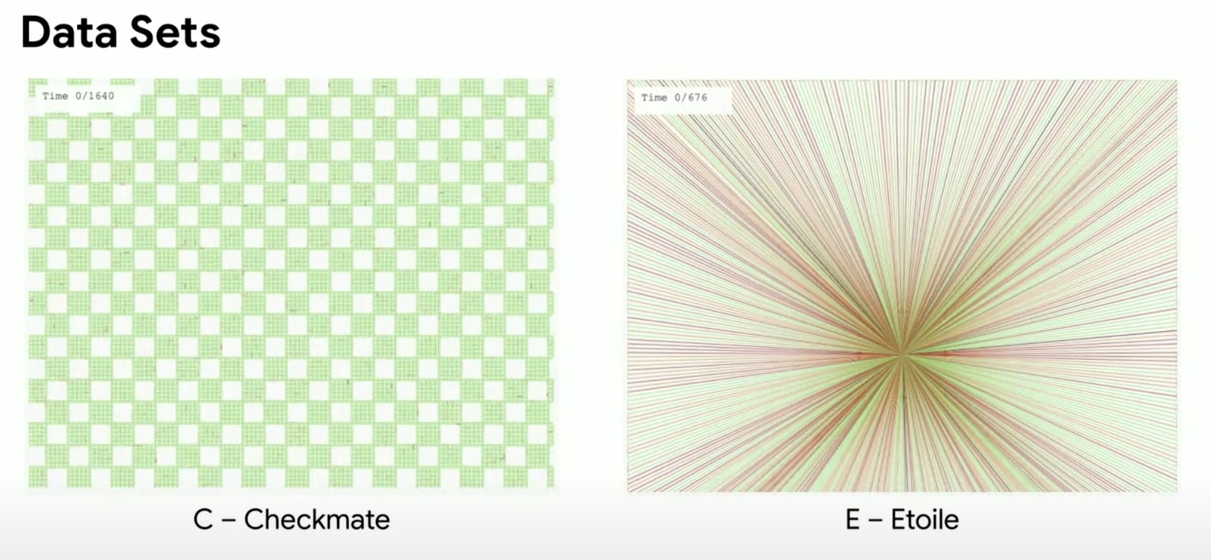
\includegraphics[width=.8\linewidth]{img/screenshots/hashcode_datasets_c_e.png}
    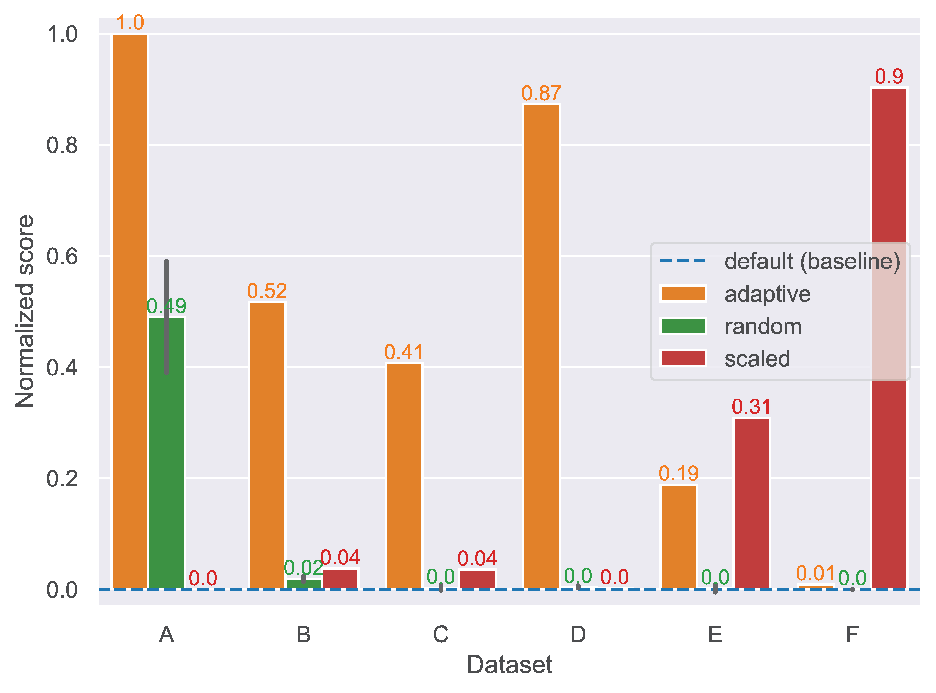
\includegraphics[width=\linewidth]{img/experiments/pdfa-init_experiment.pdf}
    \caption[Comparison of initialization options]{
        Comparison of different initialization options for each dataset.
        Y-axis shows the normalized score (see Section~\ref{subsec:score_normalization}).
        The black error bars indicate the 95\% confidence intervals.
    }
    \label{fig:init_comparison}
\end{figure}

The results are shown in Figure~\ref{fig:init_comparison}.
The \textcolor{mygreen}{\textbf{random}} option performs similarly to the \textcolor{myblue}{\textbf{default}} option---since the default order is neither optimized nor intentionally poor, it is reasonable that the random order has comparable performance on average.
The \textcolor{myorange}{\textbf{adaptive}} option achieves strong results, especially on datasets B, C, and D. This is likely because streets in these datasets are mostly used by one or a few cars, making the specific order very important and the default times a suitable choice.
The \textcolor{myred}{\textbf{scaled}} option performs best on datasets E and F. Unsure about the reason for dataset E, but dataset F contains many streets used by hundreds of cars, so it makes sense to increase the green light time for these streets.

We see that using other ``smarter'' initialization methods can significantly improve the baseline solution, enabling the optimization process to begin from a much better starting point.
We decided to use \textit{adaptive order} and \textit{default times} for datasets B, C, and D, and \textit{random order} and \textit{scaled times} for datasets E and F (see Table~\ref{tab:hyperparams_datasets_specific}).

\section{Modifying the schedules} \label{sec:modifying_the_schedules}

Once the initial schedules are created, we can start modifying them using the proposed optimization algorithms.
Since the schedules format (see Section~\ref{subsec:schedules_format}) is quite complex and each intersection's schedule may have a different number of streets, operations such as crossover or mutation are applied separately for each intersection. Moreover, because the \textit{times} array depends on the \textit{order} array, any modifications to the order array must also be applied to the corresponding times array.

\section{Genetic algorithm} \label{sec:genetic_algorithm_application}

In this section, we apply the theory introduced in Section~\ref{sec:genetic_algorithm} and describe our design of the genetic algorithm, including the selection, crossover, and mutation operators, as well as the corresponding hyperparameters. We begin with this method, as the other algorithms reuse its mutation operator to generate new states.

\subsection{Selection}

For selecting individuals for reproduction, we use \textit{tournament selection} combined with \textit{elitism}. The corresponding hyperparameters are \textit{tournament size} and \textit{elitism}, which defines the percentage of top-performing individuals that are directly selected for reproduction.
\subsection{Crossover}

For each intersection, we randomly decide whether to crossover only the order, only the times, or both. We use \textit{order crossover (OX)} for modifying the order, and \textit{two-point crossover} for modifying the times. Crossover is performed with a probability defined by the hyperparameter \textit{crossover probability}.

\subsection{Mutation} \label{sec:mutation_application}

For each intersection, we randomly decide whether to mutate only the order, only the times, or both. We use \textit{index shuffle} for modifying the order, and for the times, we add or subtract one to some values at random. Mutation is performed with a probability defined by the hyperparameter \textit{mutation probability}. When mutation is applied, the hyperparameter \textit{mutation bit rate} controls how likely each individual value is to be modified. It can be given either as a probability or as an integer specifying the expected number of modified values in the state.

\bigskip

The remaining hyperparameters of the genetic algorithm are \textit{population size} and \textit{generations}---their names are quite self-explanatory. Together with the crossover and mutation probabilities, these hyperparameters control the total number of fitness evaluations (i.e., simulation runs) performed by the algorithm.
Additionally, utilizing the approach from Section~\ref{sec:parallelization}, we run fitness evaluations within each population in parallel.

\section{Hill climbing} \label{sec:hill_climbing_application}

As explained in Section~\ref{sec:hill_climbing}, we use a variant of the algorithm that generates next states randomly because there is no explicit neighborhood structure. We simply apply the mutation operator from the genetic algorithm (see Section~\ref{sec:mutation_application}) to generate the next state. Note that we again use the hyperparameter \textit{mutation bit rate} but not the mutation probability because the mutation is always applied. The only other hyperparameter is \textit{iterations}, which sets the number of iterations the algorithm runs for.

\section{Simulated annealing} \label{sec:simulated_annealing_application}

Introduced in Section~\ref{sec:simulated_annealing}, this algorithm uses the same strategy to generate next states as presented in Section~\ref{sec:hill_climbing_application}. That means it has the same hyperparameters \textit{mutation bit rate} and \textit{iterations}. The only additional hyperparameter is \textit{initial temperature}, which sets the initial temperature of the cooling schedule. For the cooling schedule, we use a linear decay. It is defined as
\begin{equation}
    schedule(t) = \tau_{init} \cdot \left(1 - \frac{t}{T}\right) + \varepsilon,
\end{equation}
where $\tau_{init}$ is the \textit{initial temperature}, $t$ is the current iteration, and $T$ is the total number of \textit{iterations}.
% Both of these values are hyperparameters, with the initial temperature especially requiring careful tuning for each dataset to achieve good results.

\section{Hyperparameter search} \label{sec:hyperparameter_search}

Performance of all three aforementioned algorithms largely depends on the setting of their hyperparameters.
To find the best hyperparameters for the experiments, we use a form of \textit{greedy search}. That is, we only focus on optimizing one hyperparameter at a time and try to find the best value for it. Other hyperparameters are currently fixed---either heuristically or set to their already optimized values.
We test a number of reasonable values for each hyperparameter and perform runs with additional values if the results are not satisfactory.
Each setting is tested on 10 different fixed seeds and the results are averaged.

To maintain comparability, we allocate an equal budget of fitness evaluations to all three algorithms. For hill climbing and simulated annealing, this budget is easily enforced via the \textit{iterations} hyperparameter. For genetic algorithm, the number of evaluations is stochastic and cannot be precisely set; however, we always set the \textit{generations} hyperparameter so that the expected total number of fitness evaluations matches the predefined budget.

For each dataset, we use the best initialization options that we selected in Section~\ref{sec:initial_schedules}.

% TABLE WITH TESTED HYPERPARAMETER VALUES
\begin{table}[h]
\centering\footnotesize\sf

\begin{tabular}{l@{\hspace{0.5cm}}c}
% \toprule
% \multicolumn{2}{l}{\textbf{Tested values}} \\
Crossover probability & $\{0.2, 0.3, \ldots, 0.8\}$ \\
Mutation probability & $\{0.1, 0.2, \ldots, 1.0\}$ \\
Tournament size & $\{2, 3, \ldots, 10\}$ \\
Elitism & $\{0, 0.05, 0.1, \ldots, 0.3\}$ \\
Population size & $\{10, 20, \ldots, 100\}$ \\
% \midrule
Mutation bit rate & $\{1, 2, \ldots, 20\}$ \\
Initial temperature & many values between $0.1$ and $500$ \\
% \bottomrule
\end{tabular}

\caption[Tested hyperparameter values]{Ranges of tested hyperparameter values.}
\label{tab:hyperparams_tested_values}
\end{table}

To give a clearer picture of the values explored, Table~\ref{tab:hyperparams_tested_values} summarizes the ranges used in the hyperparameter search.
The genetic algorithm parameters---\textit{crossover probability}, \textit{mutation probability}, \textit{tournament size}, and \textit{elitism}---were tested only on smaller datasets E and B to reduce search complexity, because they seemed generalizable across datasets. Other parameters, especially the \textit{mutation bit rate} and \textit{initial temperature}, are highly dataset-dependent and were tuned separately for each algorithm and dataset.

Finally, Tables~\ref{tab:hyperparams_shared} and~\ref{tab:hyperparams_datasets_specific} provide a detailed overview of the selected hyperparameters for the experiments. For clarity, the first table lists the hyperparameters that are shared across all datasets, while the second table shows dataset-specific hyperparameters.

% TABLE WITH SHARED HYPERPARAMETERS
\begin{table}[h]
\centering\footnotesize\sf

\begin{tabular}{l@{}c}
% \toprule
\multicolumn{2}{l}{\textbf{Genetic Algorithm}} \\
Crossover probability & 0.6 \\
Mutation probability & 0.4 \\
Tournament size & 3 \\
Elitism & 0.05 \\
\midrule
\multicolumn{2}{l}{\textbf{Hill Climbing}} \\
Iterations & 450,000 \\
\midrule
\multicolumn{2}{l}{\textbf{Simulated Annealing}} \\
Iterations & 450,000 \\
% \bottomrule
\end{tabular}

\caption[Shared hyperparameters]{Shared hyperparameters for all datasets.}
\label{tab:hyperparams_shared}
\end{table}

% TABLE WITH DATASET-SPECIFIC HYPERPARAMETERS
\begin{table}[hb!]
\centering\footnotesize\sf

\begin{minipage}[t]{0.48\textwidth}
\centering
\begin{tabular}{l@{\hspace{0.5cm}}c}
% \toprule
\multicolumn{2}{c}{\textbf{Dataset E}} \\
\midrule
Order initialization & random \\
Times initialization & scaled \\
\midrule
\multicolumn{2}{l}{\textbf{Genetic Algorithm}} \\
Population size & 90 \\
Generations & 6,667 \\
Mutation bit rate & 9 \\
\midrule
\multicolumn{2}{l}{\textbf{Hill Climbing}} \\
Mutation bit rate & 15 \\
\midrule
\multicolumn{2}{l}{\textbf{Simulated Annealing}} \\
Mutation bit rate & 5 \\
Initial temperature & 275 \\
% \bottomrule
\end{tabular}
\end{minipage}
\hfill
\begin{minipage}[t]{0.48\textwidth}
\centering
\begin{tabular}{l@{\hspace{0.5cm}}c}
% \toprule
\multicolumn{2}{c}{\textbf{Dataset B}} \\
\midrule
Order initialization & adaptive \\
Times initialization & default \\
\midrule
\multicolumn{2}{l}{\textbf{Genetic Algorithm}} \\
Population size & 10 \\
Generations & 60,000 \\
Mutation bit rate & 2 \\
\midrule
\multicolumn{2}{l}{\textbf{Hill Climbing}} \\
Mutation bit rate & 4 \\
\midrule
\multicolumn{2}{l}{\textbf{Simulated Annealing}} \\
Mutation bit rate & 1 \\
Initial temperature & 0.25 \\
% \bottomrule
\end{tabular}
\end{minipage}
\newline
\newline
\newline
\begin{minipage}[t]{0.48\textwidth}
\centering
\begin{tabular}{l@{\hspace{0.5cm}}c}
% \toprule
\multicolumn{2}{c}{\textbf{Dataset F}} \\
\midrule
Order initialization & random \\
Times initialization & scaled \\
\midrule
\multicolumn{2}{l}{\textbf{Genetic Algorithm}} \\
Population size & 50 \\
Generations & 12,000 \\
Mutation bit rate & 2 \\
\midrule
\multicolumn{2}{l}{\textbf{Hill Climbing}} \\
Mutation bit rate & 5 \\
\midrule
\multicolumn{2}{l}{\textbf{Simulated Annealing}} \\
Mutation bit rate & 3 \\
Initial temperature & 15 \\
% \bottomrule
\end{tabular}
\end{minipage}
\hfill
\begin{minipage}[t]{0.48\textwidth}
\centering
\begin{tabular}{l@{\hspace{0.5cm}}c}
% \toprule
\multicolumn{2}{c}{\textbf{Dataset C}} \\
\midrule
Order initialization & adaptive \\
Times initialization & default \\
\midrule
\multicolumn{2}{l}{\textbf{Genetic Algorithm}} \\
Population size & 20 \\
Generations & 30,000 \\
Mutation bit rate & 2 \\
\midrule
\multicolumn{2}{l}{\textbf{Hill Climbing}} \\
Mutation bit rate & 4 \\
\midrule
\multicolumn{2}{l}{\textbf{Simulated Annealing}} \\
Mutation bit rate & 2 \\
Initial temperature & 0.1 \\
% \bottomrule
\end{tabular}
\end{minipage}
\newline
\newline
\newline
\begin{minipage}[t]{0.48\textwidth}
\centering
\begin{tabular}{l@{\hspace{0.5cm}}c}
% \toprule
\multicolumn{2}{c}{\textbf{Dataset D}} \\
\midrule
Order initialization & adaptive \\
Times initialization & default \\
\midrule
\multicolumn{2}{l}{\textbf{Genetic Algorithm}} \\
Population size & 40 \\
Generations & 15,000 \\
Mutation bit rate & 2 \\
\midrule
\multicolumn{2}{l}{\textbf{Hill Climbing}} \\
Mutation bit rate & 2 \\
\midrule
\multicolumn{2}{l}{\textbf{Simulated Annealing}} \\
Mutation bit rate & 2 \\
Initial temperature & 0.1 \\
% \bottomrule
\end{tabular}
\end{minipage}

\caption[Dataset-specific hyperparameters]{
    Dataset-specific hyperparameters.
    The order and times initializations are the same for all three methods for each dataset.
}
\label{tab:hyperparams_datasets_specific}
\end{table}
